% \chapter{Literature Survey}
% The literature survey is a broad and shallow account of the field, which helps to place the contribution of the paper in context. It is part of the motivation of the paper, because it helps to identify the gap that this work is trying to fill, and explain why it is important to fill this gap. Rather than a list of disconnected accounts of other people's work, you should try to organise it into a story: What are the rival approaches? What are the drawbacks of each? How has the battle between different approaches progressed? What are the major outstanding problems? (This is where you come in.) 


\chapter[Literature Survey and Background]{Literature Survey and\\Background}
\label{sec:background}
This chapter contains two main sections, Sports- and Exercise Science, and Algorithms.
The sports- and exercise science section will cover the necessary aspects of physical training that appear in this thesis as well as a literature survey of cases where AI has been used for training planning.
The algorithms section covers the main concepts that are used in our model GERT that is presented in \cref{sec:GERT}.

\section{Sports- and Exercise Science}
To begin with, quantification and planning of general physical training will be covered.
The section then briefly describes training in a swim-specific setting.
Finally, we present articles where AI has been applied in a training planning scenario.

\subsection{Quantifying Training}
Training is typically quantified in three ways; volume, intensity and frequency~\cite{smith2003framework}.
Volume refers to the amount of work that is performed by the athlete during a training session.
This can be measured in multiple ways, such as time of training, repetitions performed or distance traveled. 
What measure is used depends on the sport and purpose of the training.
In swimming, kilometers is often used as the measure for volume.

The intensity measures the rate of exhaustion for the work being performed~\cite{smith2003framework}.
Work at different intensities will use different energy sources and can be maintained for different durations.
In endurance training and endurance sports, intensity is often split into zones.
Training in lower-intensity zones will typically be cardio work with longer duration, while work in higher intensity zones is performed as sprints or high-intensity intervals.
The method to determine in which zone the volume is being accumulated differs between sports.
Three examples of such methods are the Rate of Perceived Effort (RPE)~\cite{borg1982psychophysical}, where the athlete will self-assess how hard the work was; measuring the percentage of maximum heart rate; or measuring the concentration of lactic acid in the athlete's blood.
In swimming, the generally adopted method is to use the speed at which the athlete is swimming. It corresponds well to the concentration of lactate in the blood, which can not conveniently be measured directly during the training~\cite{chatard1999training}.
Both the alternatives of using heart rate or RPE are ill-suited for swimming due to the slack in heart rate making up a large fraction of the relatively short training intervals and RPE being highly subjective and requiring active reporting from the athletes.

Further, it is common to see a polarized pattern of how much volume is accumulated in the different intensity zones.
Most of the training is done at low intensity and high intensities, while little work is done at moderate intensities \cite{seiler2006quantifying}.

Lastly, the frequency of training measures how often the athlete is training.
This is typically measured as how many training sessions the athlete is performing during a certain week, or for some athletes how many days they are resting.

By combining these measures it is possible to assess how hard an athlete is training.
Although no single measurement has been adopted by the scientific community, there are measurements that combine volume and intensity, to quantify how hard a training session was, which are often used~\cite{halson2014monitoring}.
An example of this is the training impulse score TRIMP developed by Banister~\cite{morton1990modeling}.
In its simplest form, the TRIMP score for a session is calculated as
\begin{equation}
    \text{TRIMP} = D \cdot \Delta \text{HR} \cdot e^{xb} \,,
\end{equation}
where $x = \Delta \text{HR} = ({\text{HR}_{ex}-\text{HR}_{rest}})/({\text{HR}_{max}-\text{HR}_{rest}})$, $\text{HR}_{ex}$ is the average heart rate for the session, $\text{HR}_{rest}$ is the athletes resting heart rate , $\text{HR}_{max}$ is the athlete's maximum heart rate, $D$ is the duration of the session, and $b$ is a weighting factor representing increased levels of blood lactate at high intensities.
% The score has since been extended to calculate the load of each intensity zone individually.
Further, there are several other proprietary measures such as TrainingPeaks' Training Stress Score\texttrademark{} (TSS)\footnote{\href{https://help.trainingpeaks.com/hc/en-us/articles/204071944-Training-Stress-Scores-TSS-Explained}{Link to Training Peak's Explanation of TSS}}, which is commonly used by cyclists.

In swimming literature, the term \textit{training load} is commonly used and refers to a TRIMP-like metric which is calculated by multiplying the training volume, measured in distance, with a coefficient based on the intensity of the swimming~\cite{chatard1999training}. The training load $w$ of a session is calculated as 

\begin{equation}
    w = \sum_{i \in I} c_i V_i
\end{equation}

where $I$ represents the different intensity zones, $c_i$ is the weight of the zone and $V_i$ volume in \si{\kilo\meter}.

% According to him, the traditional way of measuring intensity with heart rate is a bad fit for swimming, and an easier and more reliable way is to measure it using the pace of swimming.

\subsection{Modeling Performance}
\label{sec:modeling_performance}
Since the goal of training is to increase performance, it is desirable to know how one affects the other.
One of the more prevalent models for measuring the performance of an athlete is the Banister model~\cite{calvert1976systems}. 
In this model, the performance of an athlete is described as a difference between the athlete's fitness and their fatigue. 
A training session will induce both fitness and fatigue.
The values of both fitness and fatigue will decay over time, but fatigue, with a higher decay rate, will return to base values faster than fitness.
This allows the athlete to increase their modeled performance over time.
An example of the use of the model can be seen in \cref{fig:banister_example}

\begin{figure}[ht]
    \centering
    \begin{subfigure}[t]{0.48\textwidth}
        \centering
        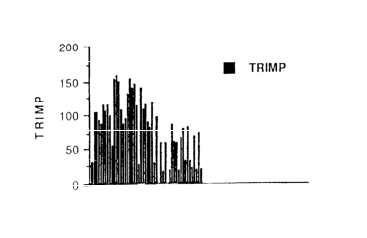
\includegraphics[width=\textwidth]{chapters/figures/background/banister1.pdf}
        \captionsetup{width=.9\linewidth}
        \caption{An athlete performs exercises that induce a response measured in TRIMP.}
    \end{subfigure}%
    ~ 
    \begin{subfigure}[t]{0.48\textwidth}
        \centering
        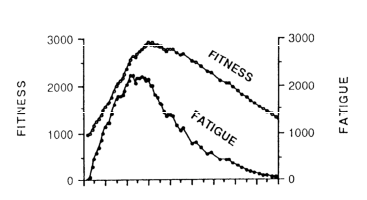
\includegraphics[width=\textwidth]{chapters/figures/background/banister2.pdf}
        \captionsetup{width=.9\linewidth}
        \caption{The fitness and fatigue that is induced by the training, note the decaying effects.}
    \end{subfigure}\\[1ex]
    \begin{subfigure}[t]{0.48\textwidth}
        \centering
        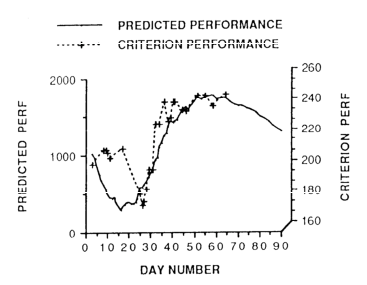
\includegraphics[width=\textwidth]{chapters/figures/background/banister3.pdf}
        \captionsetup{width=.9\linewidth}
        \caption{The predicted performance of the athlete.}
    \end{subfigure}
    \caption{An example of the use of the Banister model. An athlete performs exercises measured in TRIMP (a), which will induce both fitness and fatigue (b). The predicted performance is the difference between the curves (c). The illustrations are taken from Morton (1990)~\cite{morton1990modeling}}
    \label{fig:banister_example}
\end{figure}


The Banister model has been developed further by Busso who introduced a third term $k_3$ to the model which adds non-linearity~\cite{busso2003variable}. Using the Busso model, the performance at time $n$ is calculated as

\begin{equation}
    \hat{p}_n = p^\ast + k_1 \sum_{i+1}^{n-1} w^i e^{-(n-1)/t_1} - \sum_{i=1}^{n-1} k_2^i w^i e^{-(n-1)/t_2}
    \label{eq:busso_model}
\end{equation}
where
\begin{equation}
        k_2^i = k_3 \sum_{j=1}^i w^j e^{-(i-j)/t3}
\end{equation}

$p^\ast$ is the basic level of performance and $w^i$ is the training load from sessions $i$. $k1,k3$ represent the response in the athlete, $t1,t2,t3$ represent time decay, all these parameters are found by fitting the model to training data using the least-squares method.

This model has after its development been used to model performance and simulate optimal tapering patterns in swimmers~\cite{thomas2008model, thomas2009computer}.

\subsection{Planning}
Periodized training plans of elite athletes are traditionally split up into three layers; macro-, meso- and microcycles~\cite{bompa1983theory}.
A \textit{macrocycle} is the longest of the three and has a period of multiple months.
It is typically made up of three, smaller, \textit{mesocycles} called the accumulation phase, the specific phase and the tapering phase.
These are further split up into \textit{microcycle} with a period of about a week~\cite{smith2003framework}.

During the first mesocycle, the accumulation phase, the athlete focuses on general fitness and high volume training.
This is followed by the specific phase where the focus shifts to requirements that are specific to the type of event that an individual competes in.
This could for example be technical exercises specific to \SI{50}{\meter} butterfly swimming, if that is what the athlete competes in.
The last period of the macrocycle consists of a tapering period where the training volume is tapered to reduce stress on the body and allow recovery leading up to an event or the next macrocycle.

When the more general training plans of the macro- and mesocycles are in place the next step is to create a detailed plan for the microcycle. 
This training plan should include information on what training sessions should be performed, and in what order to obtain the specified training load.
It should also be consistent with everything already defined in the higher-level plans.
This includes having the correct number of training sessions, having the training focusing on the correct areas and arranging sessions in a way that allows for recovery between sessions.

\subsection{Training for Swimmers}
% Training for swimmers specifically is described by Chatard in~\cite{chatard1999training}.
% Training cycles for swimmers periodically alternate between high and low training loads, typically ending with a tapering period leading up to a competition.
% The tapering period focuses on reducing the fatigue of the athlete, leading to improved performance, in accordance with the described performance models.


% This has led to suggestions of block periodization with specialised mesocycles. 
% By doing this, skills are developed sequentially instead of simultaneously. 



% Mujika et al.~\cite{mujika1995effects} measures volume, frequency and intensity for several swimmers for all training sessions during a season.
% Mean intensity of the season is found to be a positive correlation to performance for swimmers who improve their personal best.
% Several articles describe how training load affects the performance of swimmers.


% Mujika~\cite{mujika1996modeled} use the training load described in \cite{chatard1999training} to model the relative performance of swimmers.
% The Banister model of fitness and fatigue is applied to predict the race results of swimmers.



An elite swimmer will typically swim between \SIrange{10}{20}{\kilo\meter\per\day}, depending on which phase of the training cycle they are currently in, with the volume spread out over 2-3 sessions per day~\cite{chatard1999training, mujika1995effects}.
Furthermore, workouts are typically structured in such a way that only the power systems or skills required are trained at a certain time. 
Hence, each training session for a swimmer has a \textit{main set}.
This main set describes the attribute or skill that is being trained during that session.
This can for example be distance training at lower intensities or intervals at race pace.
What the different types are and how often they will be performed varies depending on the coach.
The types of sessions that are used in this study will be described in the implementation section.

\subsection{ML/AI for training}
Both the Banister and Busso models, which are described in \cref{sec:modeling_performance}, have been used to generate optimal macro plans for athletes. 
Kumyaito et al. use the Busso model to develop a planner based on genetic algorithms to generate macroplans for amateur athletes~\cite{kumyaito2016intelligence}. 
Each session is defined in terms of average heart rate and duration.
The TRIMP score of each session is then used in the Busso model~\cref{eq:busso_model} to assess the performance increase of an athlete.
A limitation of the model is that it does not take physiological constraints into account. 
Hence, the model did not produce training plans that were feasible for an athlete to perform.

In 2018 Kumyaito et al. extended the idea of using the Busso model to create macro plans to include physiological constraints~\cite{kumyaito2018planning}. 
The authors use adaptive particle swarm optimization to find an optimal training plan for road cyclists.
% These constraints include monotonic training and chronic training load ramp rate.
Taking constraints into account ensure that the training is both varied and not increased too fast, both of which have been shown to lead to overtraining.
The plans are then compared to plans from British cyclists and the results show an increased performance according to the Busso model.

% Another approach is to, instead of evaluating an entire training plan, generate one session at a time given past training.
% Based on this approach Silacci et al.~\cite{silacci2019designing} design a reinforcement learning-based e-coach.
% The idea is that the e-coach should be able to adapt the training based on the current fitness of the athlete to prevent overtraining and injury.

In contrast to the generation of macro-plans as in the previous examples, there have also been attempts to generate detailed weekly training plans.
These training plans contain information not only about what training load a session should but also what exercises should be performed. 
The models are briefly described here, and an in-depth comparison to our work is made in \cref{sec:related_work}.

Skerik et al. create an automated training planner for kickboxers using numerical planning~\cite{skerik2018automated}. 
They focus solely on the general fitness period of training.
The fitness of an athlete is assessed through a series of tests.
The goal is then to create a training plan of which types of sessions to perform to increase their overall performance.
Hence, an athlete who tested poorly in some aspect will get more sessions to improve in that area.
Since the generated training plan only includes session types, they are assessed qualitatively by a coach with domain expertise.
The results of the evaluation indicate that the generated training plans are of good quality and could be of help to a coach.

Another approach where historical training sessions are used to generate new training plans for two cyclists and one runner can be found in Fister et al.~\cite{fister2019generating}.
Historical training sessions of the athlete are clustered based on average heart rate and intensity of a session.
Each cluster is then represented by a \textit{base session} that corresponds to the mean heart rate and duration of said cluster.
Six different stochastic optimization algorithms are then tested to find the number of base sessions that maximizes the TRIMP score, given constraints for the maximum average heart rate of the base sessions and the number of base sessions for the week.
The base sessions are then spread out across the week to achieve as much variation as possible, and the historical sessions from the clusters are picked such that the TRIMP score is maximized.
The results show that the model in some cases can generate plans which correspond to a \SI{90}{\percent} match with the training load of a human coach.

\section{Algorithms}
In this section, the algorithmic background for the developed system will be presented, starting with an overview of the Random Forest Regressor Chain followed by a description of the canonical genetic algorithm.

\subsection{Random Forest Regressor Chain}
\label{sec:regressor_chain}
Regression is when a statistical model is used to determine the relationship between an outcome variable and a set of feature variables.
One of the most well known of these models is the Random Forest Regressor, which utilizes a large number of bootstrapped Decision Trees to make its predictions.
This means that a large number of Decision trees are independently trained on random sub-samples of the training data, and the predictions of these trees are then weighted together to make a final prediction.
A shortcoming of this model is that it only supports scalar predictions.
If the dimensions of the outcome variable are interdependent, then multiple Random Forest Regressors, one for each dimension, will not be able to reproduce this behavior.

One way of dealing with this is to introduce a model chain as described in~\cite{read2011classifier}.
The idea is that the outcome of one regressor model is used as a feature for another.
Thus, each feature $Y_i$ is predicted sequentially and the output for each prediction is then fed back into the next regressor as input.
This gives the models the possibility to capture acyclic dependencies between the dimensions of the outcome variable.
The concept is illustrated in \cref{fig:regressor_chain_illustration}
For the case of training planning, this could help capture patterns where the training on the previous day affects the next one.

\begin{figure}
    \centering
    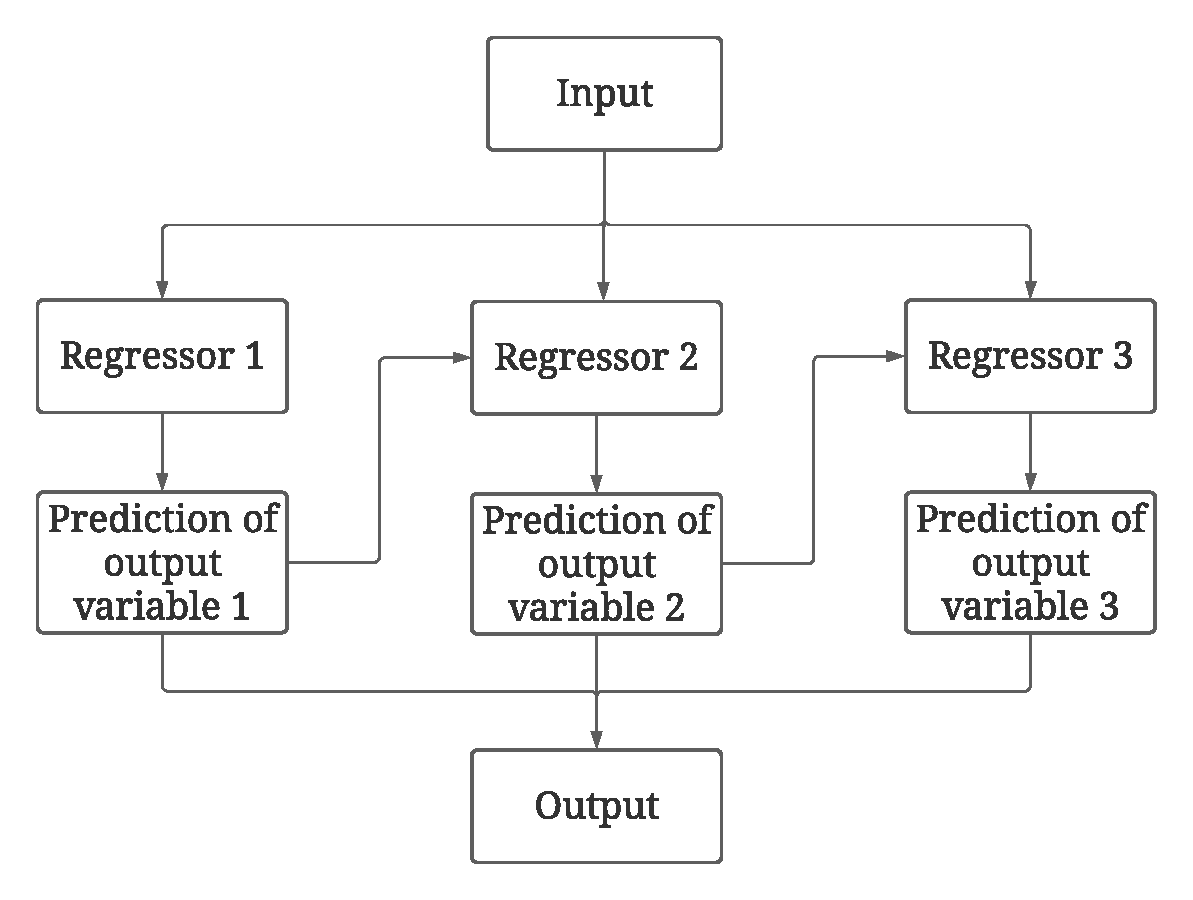
\includegraphics[width=0.8\textwidth]{chapters/figures/background/regressor_chain_illustration.pdf}
    \caption{An illustration of regressor chains. The output of each regressor is fed into the next one as an additional input variable.
    Once all predictions have been made, the outs are combined into a final prediction.}
    \label{fig:regressor_chain_illustration}
\end{figure}

\subsection{Genetic Algorithms}
\label{sec:genetic_algorithms}
Genetic algorithms, introduced by Tom Holland in 1975, are population-based evolutionary algorithms aimed at mimicking natural selection processes~\cite{holland1992adaptation}.
The algorithm starts by creating a random population.
An intermediate population is created based on a selection process.
From the intermediate population, the next generation is created using crossover and mutation operations~\cite{whitley1994genetic}.

\begin{algorithm}[H]
\SetAlgoLined
\KwResult{The best gene}
 Initialize population\;
 \While{Termination criteria is not met}{
  Selection\;
  Crossover\;
  Mutation\;
 }
 \caption{A generic genetic algorithm.}
\end{algorithm}

The selection phase assigns a fitness score to each sample of the population based on a goal function.
It is up to the user to define the goal function that the algorithm will optimize.
The fitness score is typically assigned relative to the rest of the population.
When assigned, it is the determining factor for whether a sample will live on to reproduce and be a part of the next generation.
Whitley\cite{whitley1994genetic} describes a process where the chance of a sample making it to the next generation is equal to the relative fitness score.
For example, if sample $p_i$ has a relative fitness score $f_r( p_i ) = f(p_i) / \Bar{f} = 1.36 $, where $\Bar{f}$ is the average fitness score of the population, then $p_i$ will have a \SI{100}{\percent} chance of having one sample in the intermediate population and a \SI{36}{\percent} chance of having two.

The crossover is the recombination phase of two samples.
Two parents are randomly selected from the intermediate population.
Two children are then produced by 1-point, 2-point or uniform crossover.
The crossovers are illustrated in \cref{fig:crossover_example}.
In a 1-point crossover, a line is drawn at a random position of a sequence.
The data points on the left side will come from one parent while the points on the right side will come from the other.
In a 2-point crossover, a span is generated instead. The data points inside of the span will be taken from one parent, while those on the outside are taken from the other.
Alternatively, each data point can be decided by sampling from a uniform Bernoulli distribution.
This is called uniform crossover.


\begin{figure}
    \centering
    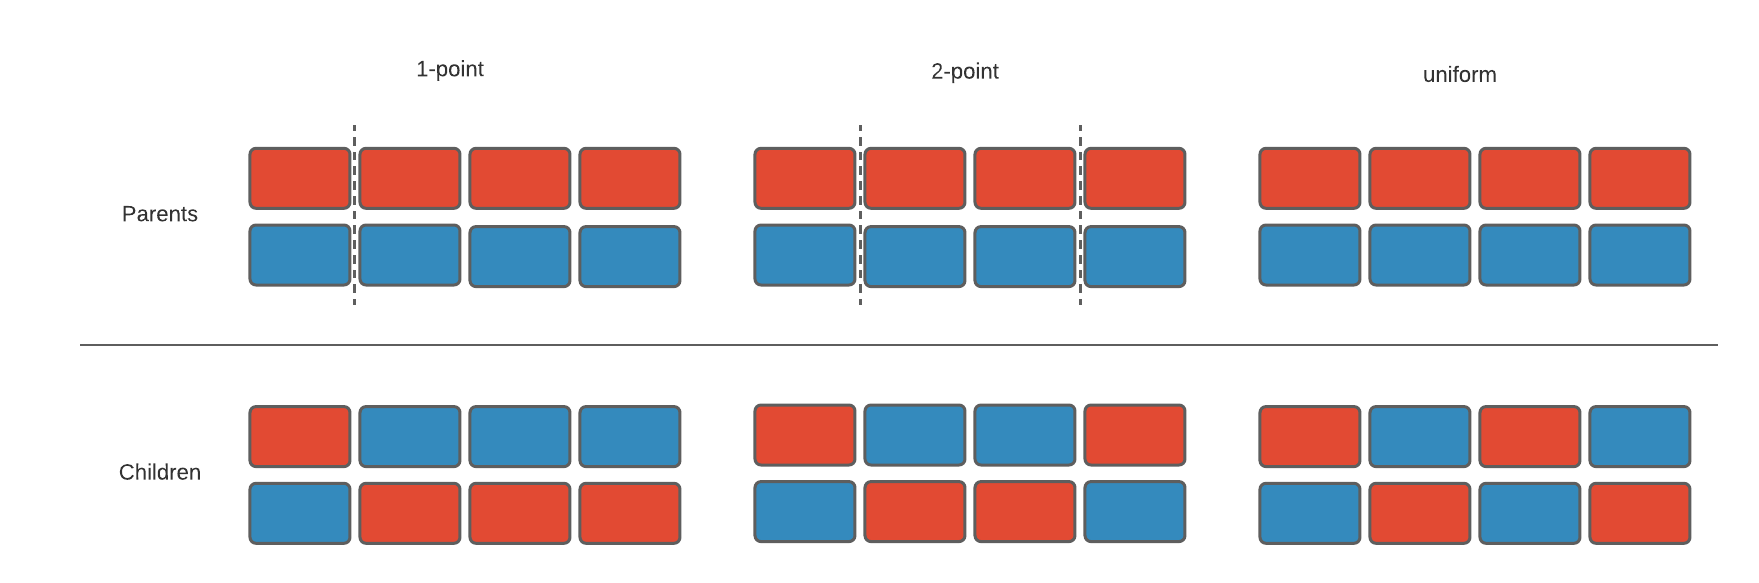
\includegraphics[width=\linewidth]{chapters/figures/ga_crossover_example.png}
    \caption{Different genetic algorithm crossovers. From the left; 1-point, 2-point and uniform crossover are illustrated.}
    \label{fig:crossover_example}
\end{figure}

The last part of the genetic algorithm is the mutation of genes.
The mutation can be done in different ways, either by drawing a completely new sample or by replacing a single data point in the sample.
